% Abstract for this chapter
%
%**********************************************************************

% %%%%%%%%%%%%%%%%%%%%%%%%%
% \section{Background}
% %%%%%%%%%%%%%%%%%%%%%%%%%


%%%%%%%%%%%%%%%%%%%%%%%%%
\section{Space robots}
%%%%%%%%%%%%%%%%%%%%%%%%%
%
% ---------------------------------------------------------------------
\begin{figure}[t]
  \centering
  \begin{minipage}{0.45\linewidth}
    \centering
    \includegraphics[width=1.0\linewidth]{fig/chapter1/canadarm.eps}
    \footnotesize\par{(a)}
  \end{minipage}
  \hspace{2mm}
  \begin{minipage}{0.45\linewidth}
    \centering
    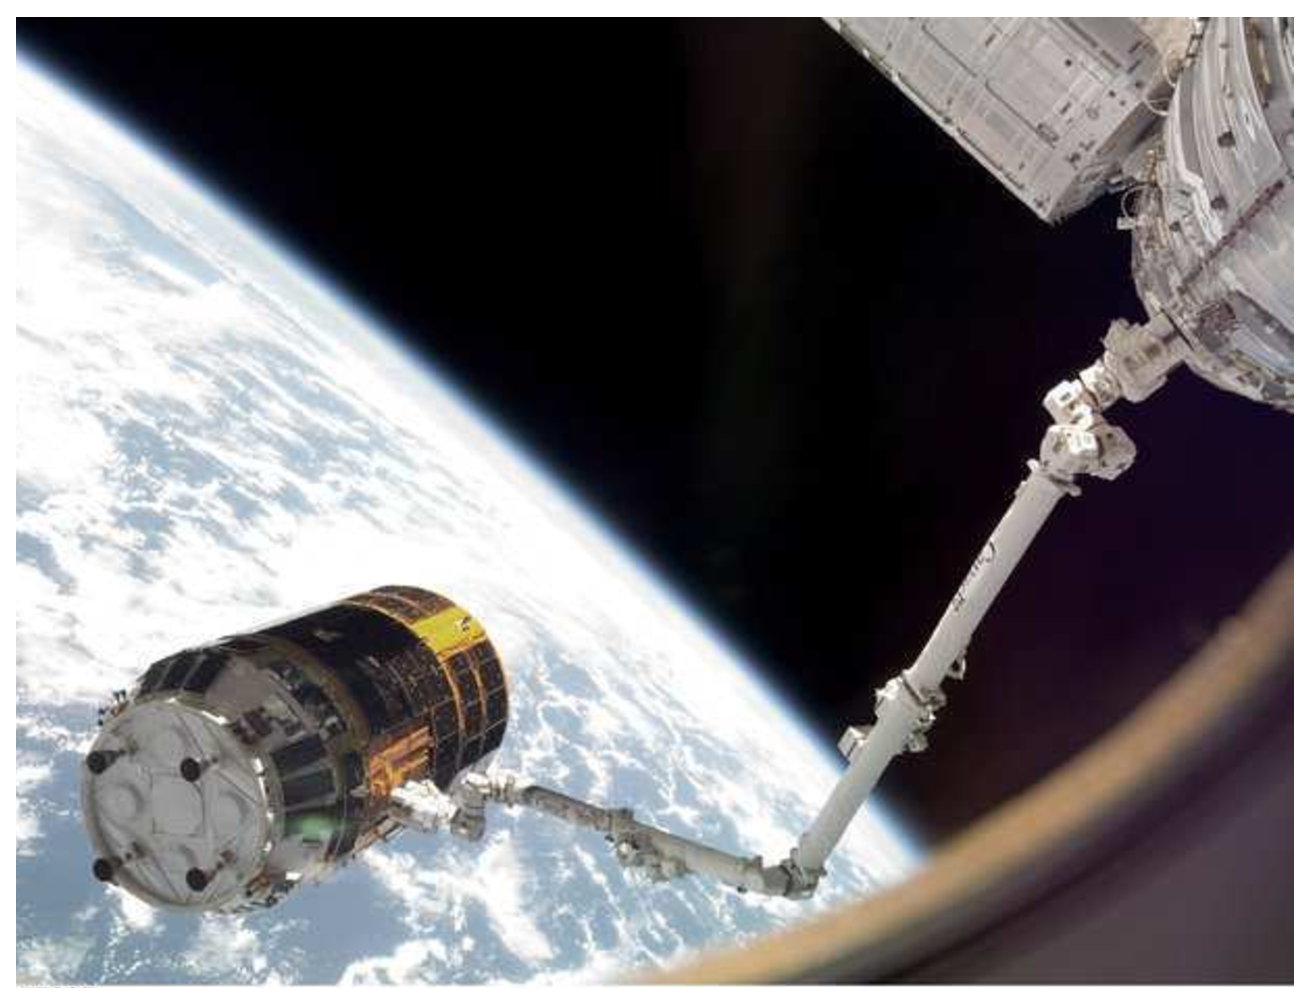
\includegraphics[width=1.0\linewidth]{fig/chapter1/canadarm2.eps}
    \footnotesize\par{(b)}
  \end{minipage}\\
  \vspace{1em}
  \begin{minipage}{0.45\linewidth}
    \centering
    \includegraphics[width=1.0\linewidth]{fig/chapter1/JEMRMS.eps}
    \footnotesize\par{(c)}
  \end{minipage}
  \hspace{2mm}
  \begin{minipage}{0.45\linewidth}
    \centering
    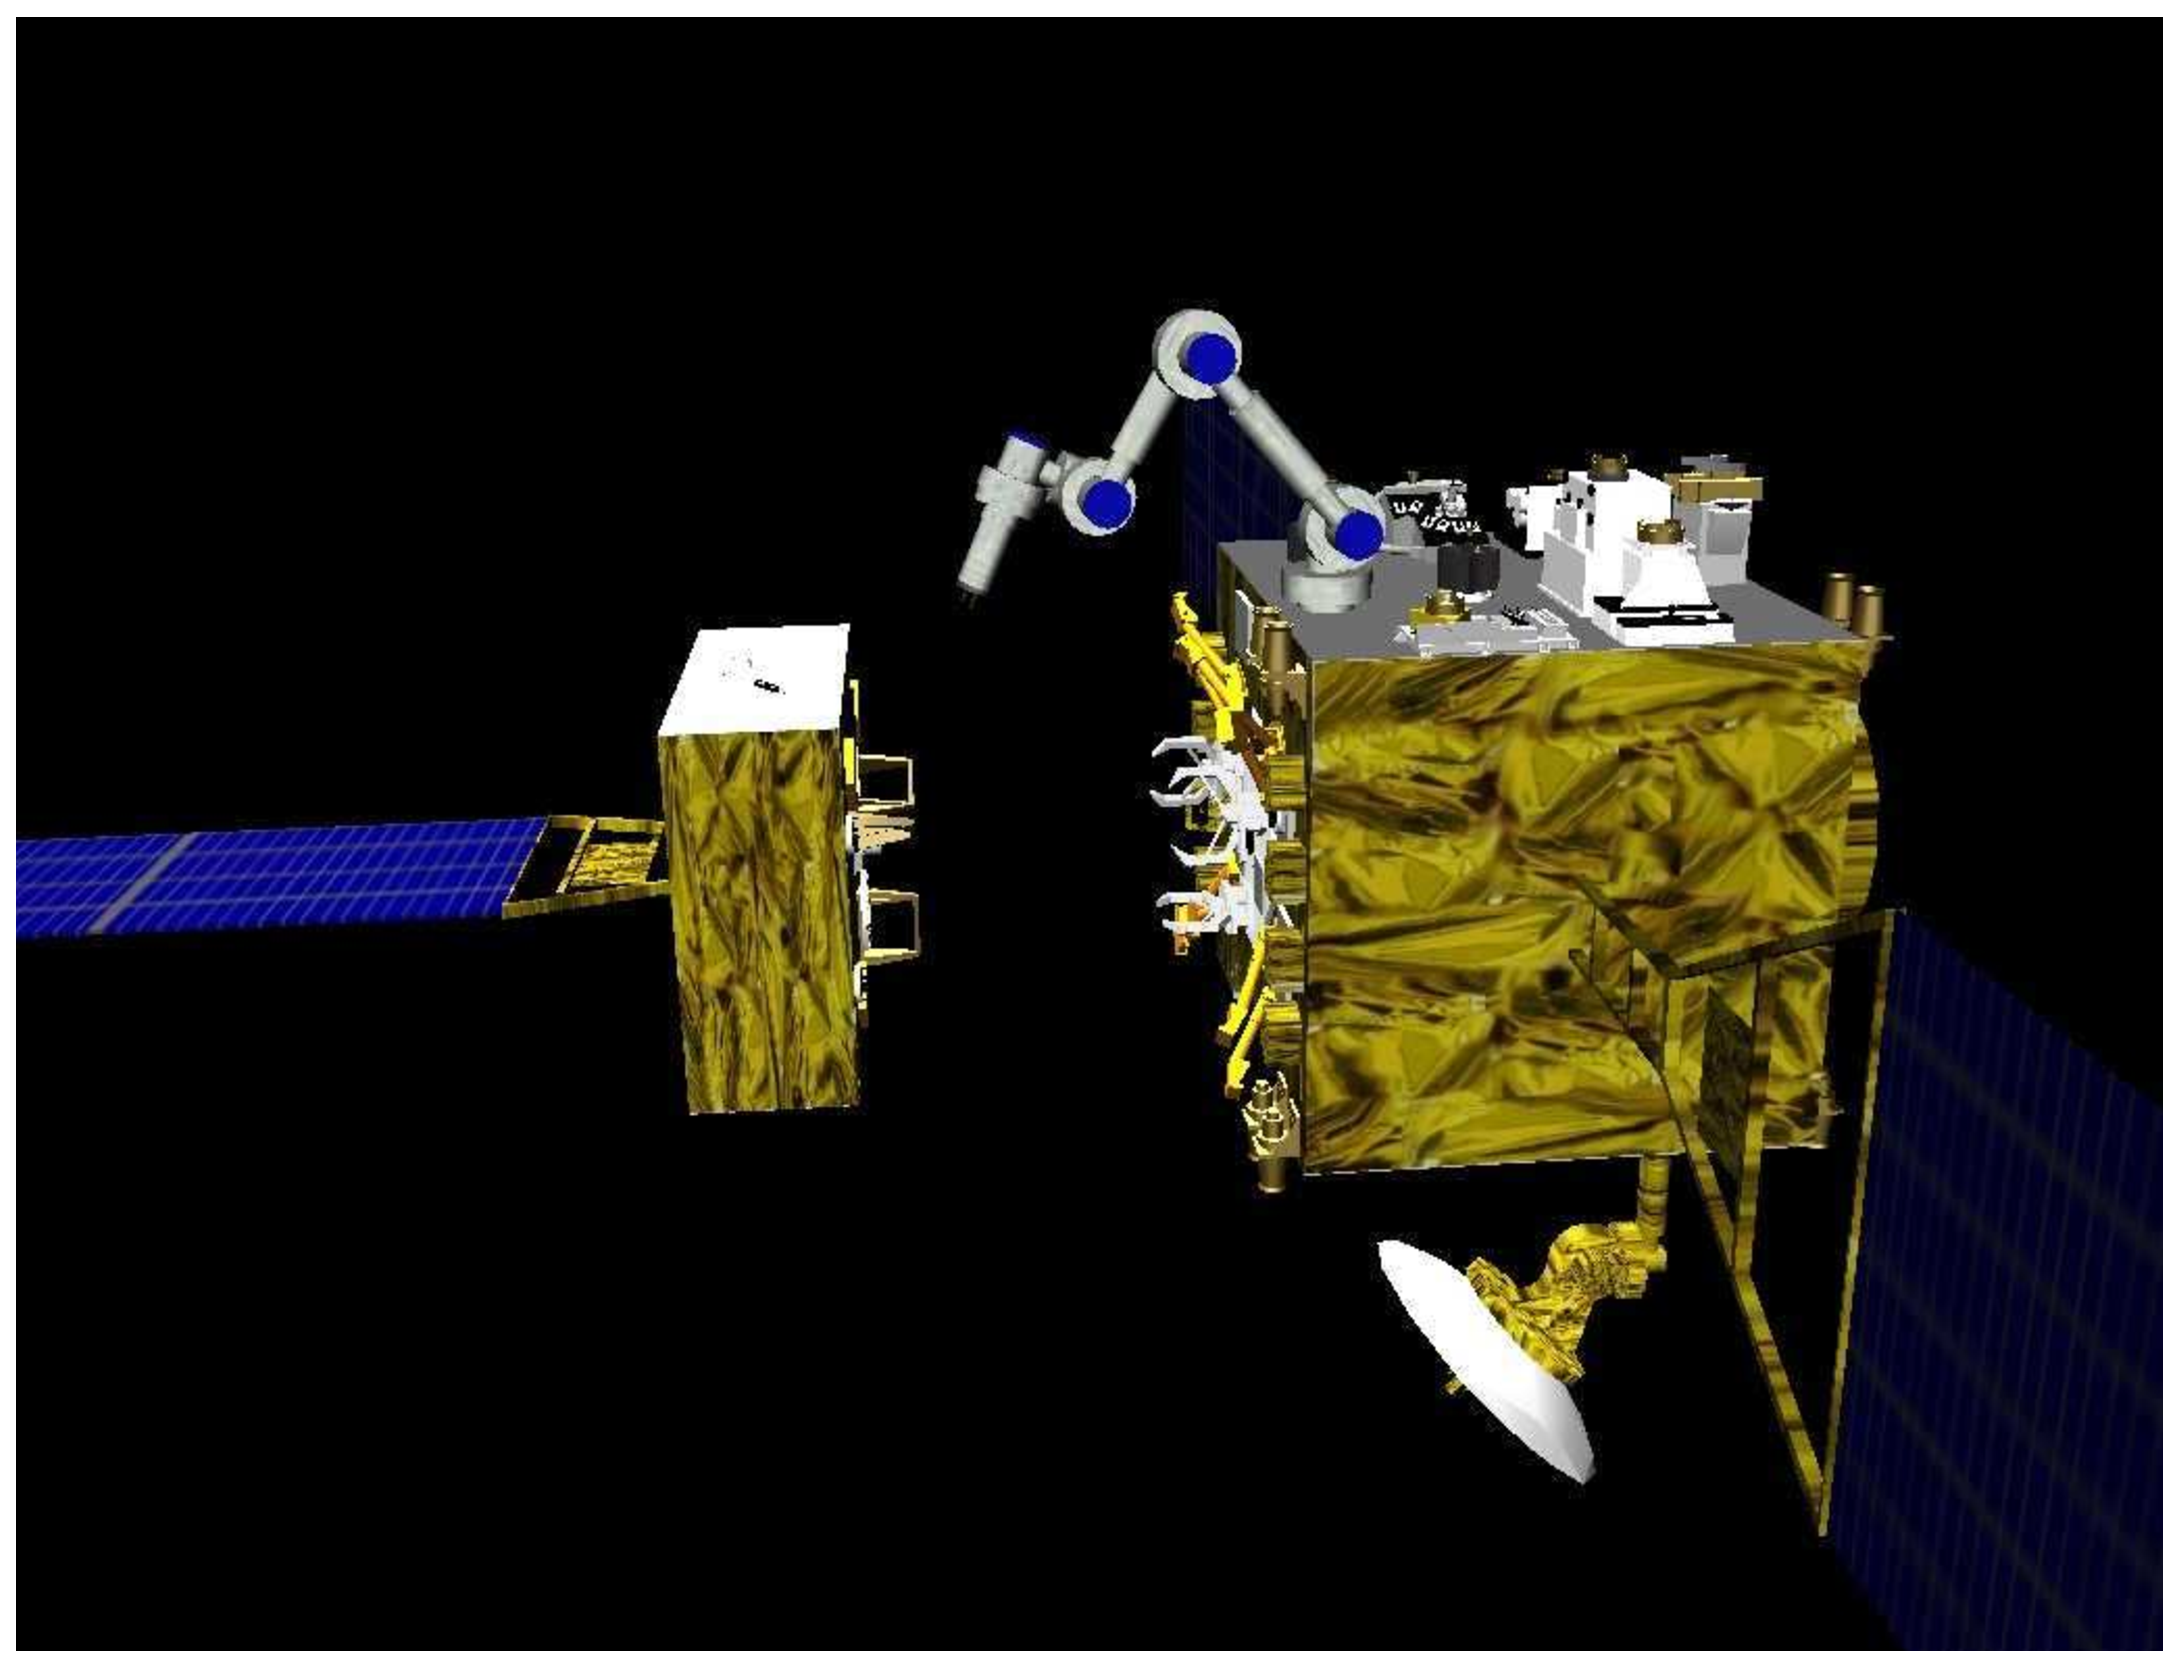
\includegraphics[width=1.0\linewidth]{fig/chapter1/ETSVII.eps}
    \footnotesize\par{(d)}
  \end{minipage}
  \caption{Space robotic systems: (a) Canadarm \copyright NASA, (b) Canadarm 2 \copyright NASA, 
    (c) JEMRMS \copyright JAXA and (d) ETS-VII.}
  \label{fig:SR}
\end{figure}
% ---------------------------------------------------------------------
%

The first use of a robotic system in space is the Shuttle Remote Manipulator System (SRMS),
whose nickname is \textit{Canadarm} (\fig{SR}~(a)),
on Space Shuttle Colombia in 1981 \cite{Flores-Abad2014}.
After that, robotic systems have been employed in various space missions.
A well-known space robot is the Space Station Remote Manipulator System (SSRMS)
developed by the Canadian Space Agency (CSA).
The manipulator was named \textit{Canadarm 2} and has performed several missions, successfully;
the most recent mission executed by Canadarm 2 is a catching mission of the H-II Transfer Vehicle (\fig{SR}~(b)).
Canadarm 2 consists of 17-meter long, 7 degree-of-freedom (DoF) symmetric mechanism.
As a similar robotic system,
the Japan Aerospace Exploration Agency (JAXA) developed the Japanese Experiment Module
Remote Manipulator System (JEMRMS) and a small fine arm (SFA) attached on the end of JEMRMS;
hence, the combined system has been referred to as JEMRMS/SFA (\fig{SR}~(c)).

In addition to this kind of space robotic system,
free-floating space robots (FFSR), which consists of a satellite base and at least one manipulator arm,
are expected to perform future space missions.
These missions would be debris removal, construction of large space buildings,
servicing for launched satellites and so on.
So far, this type of space robots have not been used in practical missions.
% Only experimental systems were developed before.
On the other hand,
an experimental robotic system was developed by JAXA around 1997.
The robotic system has been referred to as the \textit{Experimental Test Satellite VII} (ETS-VII) \cite{Oda1997}.
ETS-VII consists of a 2-meter long, 6-DoF manipulator and a 2000 kg class of unmanned satellite (\fig{SR}~(d)).
The system demonstrated some important robotic technologies:
autonomous rendezvous and docking (AR\&D) and robotic servicing.
The robotic servicing includes exchange of orbital replacement unit (ORU),
deployment of a space structure and capturing of a target satellite.
As an important results,
it was confirmed that the manipulator motions actually induced base motions
as indicated from the mechanics theory \cite{SPACEROBOT,Masutani,Yoshida2003}.
Hence, specific controller designs for space robots
have to be developed in order to execute future space missions, successfully.

%%%%%%%%%%%%%%%%%%%%%%%%%%%%%%%%%%%%%
\subsection{Control issues with FFSR}
%%%%%%%%%%%%%%%%%%%%%%%%%%%%%%%%%%%%%
The most significant problem when controlling manipulators in space
is the dynamic coupling between the manipulators and the satellite base.
The coupling induces a base translation and also rotation.
Because of the base motions,
control methods that have been employed in terrestrial robots cannot be applied straightforwardly.
To overcome this problem,
the information of the base motions has to be taken into account within the control schemes.

An important study considering the above issue was done in \cite{Masutani,Umetani1989}.
The authors proposed the Generalized Jacobian,
which includes a base motion estimated from the linear/angular momentum conservation laws.
By using the Jacobian,
the correct mapping from task space into the joint space can be obtained.
This method can be applied simply by replacing the conventional Jacobian matrix with the generalized one
on the terrestrial robot controllers.
The resolved motion rate control and the resolved acceleration control with the Generalized Jacobian were verified
through numerical simulation.
In addition,
on the experiment with ETS-VII,
the utility of the generalized Jacobian was
confirmed under resolved motion rate control \cite{Yoshida2003}.

On the other hand,
a base rotation itself is a problem because it induces a communication failure between
the space robot and the ground control center.
To overcome this problem,
using gas-jet thrusters were considered by some researchers \cite{Dubowsky1991}.
On the experiment of ETS-VII,
under a camera inspection type of mission,
the thrusters were used to stabilize the base attitude.
However, the fuel for thrusters is finite and its amount determines the life duration of the space systems.
Therefore, attitude devices using electric power such as reaction wheels have been considered so far \cite{Yoshida1994,Aghili2009}.
Reaction wheels have been successfully used on zero momentum type of various satellites
to stabilize their attitude especially against the gravity gradient torque, earth magnetism torque and
solar radiation pressure.
However, if it is considered that reaction wheels are used to compensate
the base reaction induced by a manipulator motion,
the output torque of the reaction wheels is quite insufficient with respect to the base reaction.
To avoid saturation of the reaction wheel signals,
the manipulator has to be driven at very low speed.
When some repeatable tasks, e.g.\ observation/inspection or assembly for construction missions
are performed, this low speed manipulation is
not desirable from the perspective of work efficiency \cite{Umetani1989}.
Hence, developing a control method that generates a manipulator motion inducing a small reaction
is an important issue for space robots.

A pioneering work on manipulator reaction control with free-floating manipulator systems
introduced the Disturbance map concept \cite{Dubowsky1991,Dubowsky1993}.
The base disturbance magnitude is visualized as a colored map in joint space.
With this tool, low reaction paths can be obtained in an intuitive manner.
However, it is difficult to employ this method with manipulators of more than two degrees of 
freedom (DoFs), 
In addition,
it is difficult to obtain a low reaction motion through the color map, automatically.

%%%%%%%%%%%%%%%%%%%%%%%%%%%%%%%%%%%%%%%%%%%
\subsection{Reactionless motion control}
%%%%%%%%%%%%%%%%%%%%%%%%%%%%%%%%%%%%%%%%%%%
A motion generation method was proposed for zero reaction manipulation.
This method has been referred to as the \textit{Reaction Null-Space} (RNS)
formulation \cite{Nenchev1990, Nenchev1999b, Nenchev1999a},
and provides a straightforward approach to reactionless motion generation.
Therein, the condition of reactionless motion was derived from the angular momentum conservation law.
The method was confirmed at the on-orbit experiment with ETS-VII \cite{Yoshida2001}.

In the previous studies,
reactionless motion controls based on RNS have been considered by several researchers \cite{Hirano2014,Oki2007,Hara2010}.
For instance,
the angular momentum distribution control for capturing non-cooperative satellites
under the reactionless condition was proposed \cite{Dimitrov2004}.
The capability of the method was investigated with a planar model.
With a dual arm planar model,
point-to-point (PTP) reactionless motion control was considered for capturing space debris \cite{Shah2013}.
For vibration suppression of flexible appendages on a satellite,
reactionless motion control of the end-effector was considered
in addition to the vibration suppression control \cite{Hirano2014}.
In these studies,
position control of the end-effector under reactionless motion was focused on.
However, the position control between arbitrary locations
would be impossible on general type of spatial manipulators,
e.g.\ six-DoF and seven-DoF redundant manipulators,
due to the limitation of these kinematic structures.
In fact,
the above methods were verified with planar models only.

The possibility of using the RNS method with spatial models is still uncertain, despite 
the reports on some interesting results. For example, within the extended ETS-VII mission,
simple reactionless tasks were examined \cite{Yoshida2000,Yoshida2001}.
Also, results from simulations with a modified ETS-VII manipulator model 
were presented  \cite{Yoshida2001}. In the latter study it was concluded that kinematic redundancy is 
important for the extension of the workspace under reactionless control.
For point-to-point position control, the reaction-null/Jacobian transpose controller
was proposed in \cite{Pisculli2014}. This method was verified with a dual arm 
manipulator system, each manipulator comprising  six DoFs. 
In this work, it was shown that the reachable region of the end-effector from an initial
configuration is quite narrow due to the limitation of the kinematic structure.
On the other hand, a singularity treatment method (the Singularity Consistent approach) 
 was applied to deal with  algorithmic singularities introduced by the reactionless
motion constraint \cite{Nenchev1999c}. It was also confirmed that the workspace of the end-effector 
becomes quit narrow when considering constraints imposed on both end links, the end-effector and the base.
In summary, we can conclude that position control of the end-effector under reactionless control is 
not appropriate in practical tasks even if singularity treatment techniques are used.


%%%%%%%%%%%%%%%%%%%%%%%%%%%%%%%%%%%
\subsection{Energy consumption}
%%%%%%%%%%%%%%%%%%%%%%%%%%%%%%%%%%%
As a different issue in space systems,
energy consumption has been considered.
In the case of controlling satellite attitude,
a power minimization control with redundant reaction wheels were proposed in \cite{Schaub2009}.
From the perspective of tool design,
a low-power image payload was discussed \cite{Carpenter2008,Carpenter2009}.
In that study, Control Moment Gyros (CMG) were employed
because theirs mechanical power/energy is smaller than these produced by a reaction wheel assembly.

On the other hand,
in the field of robotics,
a control method that reduces the energy consumption of free-flying space robots
was proposed \cite{Nakamura1993}.
The study assumed that the base attitude is controlled through four reaction wheels.
Then, the redundant reaction wheel was used to reduce the energy consumption
throughout a manipulator motion.
In \cite{Lampariello2013},
the mechanical power was used as a cost function that is to be minimized.

On reactionless motion control,
the energy optimum reactionless path planning was proposed \cite{Shah20132}.
The method utilized redundancy to optimize the kinetic energy of dual manipulators.
However, a rapid change of the joint velocities was observed due to the optimization.

As mentioned in \cite{Carpenter2008},
reaction wheels require high amount of mechanical power when a large output torque is generated.
Generally, when reaction wheels are used to compensate
the base reaction induced by a manipulator motion,
the reaction wheels must generate a high output torque.
Consequently, the energy consumption becomes large.
On the other hand, reactionless motion control does not necessarily need to use reaction wheels completely.
Hence, it is possible to reduce the energy consumption without
an additional optimization that usually induces unstable behaviors.
The reduction of the energy consumption when using reactionless motion control
has not been discussed before.
In this work,
we focus on the energy consumption reduction and show an interesting result.


%%%%%%%%%%%%%%%%%%%%%%%%%%%%%%%%%%%
\section{Motion/Force control}
%%%%%%%%%%%%%%%%%%%%%%%%%%%%%%%%%%%
With terrestrial robots, force control of the end-effector is as important as motion control.
Especially under interaction tasks,
whose typical examples are polishing, deburring, machining or assembly in industrial settings,
force control providing a compliance behavior
is crucial due to a safe contact between the end-effector of a manipulator and
the unstructured environments.
To understand the importance of the compliance behavior,
we consider a situation that an interaction task is executed by a motion control scheme.
In this case,
the contact between a manipulator and the environment
may cause a deviation of the end-effector motion from the desired trajectory.
Then, an appropriate position feedback controller should intend to reduce the deviation.
As a result,
a built-up of the contact force may occur until causing breakage of a part of the manipulator.
Hence, the compliance behavior of the manipulator end-effector must be needed.

This compliance behavior can be obtained through passive/active interaction control approaches.
The passive approach makes use of a specifically designed
mechanical device such as the Remote Center of Compliance (RCC) device.
This device is designed and has been used for peg-into-hole like tasks.
From the perspective of response time,
the use of a passive device is more suitable than the use of active control approaches.
However, in order to use the passive approach in industrial applications,
specific mechanical devices have to be designed for every robot task.
In addition, the passive devices can only deal with small position and orientation deviations.
Hence, to provide flexibility in robotic tasks,
active interaction control has to be developed.

The active interaction control schemes can be classified into two categories:
indirect force control and direct force control.
Impedance control is a well-known scheme belonging to the first category.
Under impedance control,
the behavior of the end-effector is modeled as an equivalent mass-spring-damper system with
adjustable parameters.
With the model, the contact force of the end-effector
can be related to the deviation of the end-effector motion from the desired one.

On the other hand,
hybrid motion/force control belonging
to the second category has been developed.
The most well-known approach is the so-called \textit{Operational Space} (OS) formulation,
which provides the dynamics of a manipulator in task-space coordinates.
% Using the method can provide a linear and decoupled behavior of the end-effector motion and force.
If the system is non-redundant,
the task-space coordinates are actually the generalized coordinates of the system.
However, with redundant manipulators,
the task-space coordinates cannot be generalized coordinates because there is infinite possibility
providing a relation between the task-space and the joint-space coordinates.
Hence, a suitable transformation between the task-space and joint-space has to be chosen.
To obtain a relation between the two spaces,
the inertia-weighted generalized inverse has been used in various studies \cite{Khatib1987,Park1999,Ott2008,Nakanishi2008}.
The inversion provides a decoupled feature between the task-space and the null-space.
This character is suitable to design task/joint spaces control systems independently of each other.
While task space behavior under the OS formulation (the inertia weighted generalized inverse) seems to be feasible,
unstable behaviors have been observed in joint space \cite{Hollerbach1985,Hollerbach1987}.
In addition, the dynamics of joint-space is to be hidden under the OS formulation.
As a result, the gravity compensation might cause
a cyclic joint motion without affecting the task-space behavior.

Because of these drawbacks of the OS formulation,
we proposed a new motion/force control scheme based on the Reaction Null Space (RNS) formulation,
which has been used for space robots,
especially for redundant manipulators \cite{Hara2012}.
The formulation can represent the dynamics in task-space coordinates without
making use of a transformation between the two spaces.
In addition, the joint motion is explicitly presented in the task-space dynamics.
Comparing with the OS formulation,
we confirmed that the RNS-based control would have an advantages in terms of joint motion \cite{Hara2012}.
In this work, we provide a depth discussion of the joint motion under the RNS-based control that
has been unclear so far.


%%%%%%%%%%%%%%%%%%%%%%%%%%%%%
\section{Aim of this study}
%%%%%%%%%%%%%%%%%%%%%%%%%%%%%
This thesis treats the following two topics for the RNS-based controls:
(i) reactionless motion control for free-floating space robots and
(ii) motion/force control for fixed-base redundant manipulators.

On reactionless motion control of free-floating space robots,
we discuss the following issues:
%
\begin{description}
\item[i-1] Analysis of reactionless motion from the perspective of nonlinear dynamics.
\item[i-2] Proposal of some practical tasks suitable for execution under reactionless motion control.
\item[i-3] Analysis of the energy consumption under reactionless motion control.
\end{description}
%

On the RNS-based motion/force control,
we treat the following topics:
\begin{description}
\item[ii-1] Obtain a specific model for the RNS-based motion/force control.
\item[ii-3] Clarify the joint motion under the RNS-based motion/force control.
\end{description}


%%%%%%%%%%%%%%%%%%%%%%%%%%%%%%%%%%
\section{Outline of this thesis}
%%%%%%%%%%%%%%%%%%%%%%%%%%%%%%%%%%
This thesis consists of the eight chapters as follows:
\cha{BASIC} describes the modeling of free-floating base robot systems.
The equation of motion of the system is derived from the Euler-Lagrange's equation.
Then, linear and angular momentum conservation laws are
derived via considering the invariance of the system Lagrangian 
with translation and rotation of the entire system.
Finally, we present the Reaction Null-Space formulation
in terms of both momentum and dynamics.

In Chapters \ref{cha:ANALYSIS} to \ref{cha:ENERGY},
we deal with reactionless motion control of free-floating space robots.
In \cha{ANALYSIS},
we provide an analysis of reactionless motion with a planar two-DoF model
from the perspective of nonlinear dynamics:
vector field, fixed point and bifurcation.
Besides, with a seven-DoF redundant manipulator,
we obtain a representation of its reactionless motion that is useful to consider
for practical reactionless tasks.

\cha{PROPOSAL} discusses motion tasks suitable for execution
under reactionless motion control.
We propose the following three tasks:
(i) inspection task using a hand camera,
(ii) point-to-point positioning task,
(iii) deployment task from a stowed configuration.
The performance of these tasks is verified via numerical simulations.

In \cha{ENERGY}, we deal with the energy consumption of free-flying space robots,
comparing that produced by reactionless motion control with that produced by reaction wheels used controllers.
Under zero base attitude deviation,
we show that reactionless motion coincides with the instantaneous energy minimum motion to a high degree.
Then, the energy consumption of reactionless motion control is compared
with a conventional controller using reaction wheels under the inspection tasks.

In the next two chapters,
we deal with the motion/force control based on the Reaction Null-Space for fixed base redundant manipulators.
In \cha{FORMULATION},
we formulate the RNS-based motion/force control.
Then, a specific model for the RNS-based controller is presented.
Finally, the performance of the proposed method is verified through numerical simulation.

\cha{JOINT} discusses the joint motion under the RNS-based motion/force control.
We show an interesting fact that the joint motion under the RNS-based controller
is equivalent to that under the resolved acceleration control.
The theoretical derivation and numerical verification are obtained.

Finally, \cha{CONCLUSION} summarizes this thesis.

%%%%%%%%%%%%%%%%%%%%%%%%%%%%%%%%%%%%%%%%%%%%
\section{The roles of variable's index}
%%%%%%%%%%%%%%%%%%%%%%%%%%%%%%%%%%%%%%%%%%%%
Basically, we describe vectors and matrices according to the following roles of the indexes.
\textit{Left superscript}: reference frames in which quantities are described.
\textit{Right superscript}: conditions of variables,
  e.g.\ $T$ (Transposed), $-1$ (Inversion), $des$ (Desired), $ref$ (Reference) and so on.
\textit{Right subscript} physical quantities, component, manipulator mechanisms and so on.

We provide two examples according to the above roles, in what follows.
First, we consider the Jacobian $\bm{J}$ associated with end-effector linear velocity $\bm{v}_{e}$
with respect to the inertial coordinate frame $\{F\}$.
This matrix is written as ${}^{F}\bm{J}_{v_{e}}$.

Next, we consider the same Jacobian but it just consists of the positioning subchain $P$,
which is a specific part of a manipulator mechanism.
This matrix is written as ${}^{F}\bm{J}_{Pv_{e}}$.
Note that if we consider the whole mechanism of a manipulator,
we omit this notation.

If we describe relative quantities such as position, velocity,
we will make use of the following notation:
$\bm{r}_{A \rightarrow B}$ representing a position vector pointing to the position $B$
with respect to $A$.
Note that the notation of the inertial coordinate frame is omitted in all quantities appearing below.



%**********************************************************************
%
%
%%% Local Variables:
%%% mode: latex
%%% TeX-master: "./main"
%%% End: